% -*- mode: LaTeX; coding: utf-8 -*-
\documentclass[12pt]{article}
\usepackage[T2A]{fontenc}
\usepackage[utf8]{inputenc}
\usepackage[russian]{babel}
\usepackage{amsmath}
\usepackage{amssymb}
\usepackage{eufrak}
\usepackage{epsfig}
\usepackage{psfrag}
\usepackage{tabularx}
\usepackage{wrapfig}
\usepackage{subfig}
\usepackage[TeXdef]{lev}
\usepackage{listings}
\usepackage{graphicx}
\lstloadlanguages{ [ LaTeX ] TeX, bash, C++, make, python}
\lstset{language=python, escapechar=|, extendedchars=true} 

\usepackage[unicode,colorlinks]{hyperref}
%\hypersetup{colorlinks=true, linkcolor=blue, filecolor=blue, pagecolor=blue, urlcolor=blue}
\hypersetup{colorlinks=true, linkcolor=blue, filecolor=blue, urlcolor=blue,
pdftitle={SYMBALG}, pdfauthor={Иванов А.В и Жданов С.А}}

\def\nil{}

%\def\sr#1{\left<#1\right>}
%\def\srt#1{\partial\left<#1\right>/\partial t}
%\def\srT#1{\dfdx{}{t}\left<#1\right>}
%\def\dfdx#1#2{ \frac{\partial #1}{\partial #2} }
%\def\pankrat{L}
%\newcommand{\rot}{{\rm rot}~}
%\renewcommand{\vec}[1]{{\mathbf #1}}
%\def\s{m}
%\def\S{\vec{\s}}
%\def\sxi{\s_{\text{x}i}}
%\def\syi{\s_{\text{y}i}}
%\def\szi{\s_{\text{z}i}}
%\def\H#1{\vec{H}^\text{#1}}

%\def\sx#1{\s_{\text{x}#1}}
%\def\sy#1{\s_{\text{y}#1}}
%\def\sz#1{\s_{\text{z}#1}}

%\def\r{\vec r}
%\def\k{\vec k}
%\def\h{\vec h}
%\def\i{\vec i}
%\def\o{\vec o}
%\def\p{\vec p}

%\usepackage{euscript}
%\def\Ef{\EuScript{E}_F}
%\def\nf{n_F}
%\def\Uw{U_{\rm wall}}
%\def\J{\EuScript{J}}

%\def\RACS{{\tt RACS}} 
%\def\racs{{\tt RACS}{ }} 
%\def\CVS{{\tt CVS}} 
%\def\opt#1{{\tt #1}} 
%\def\env#1{{\tt \$#1}}
%\def\Python{{\tt Python}}
%\def\SWIG{{\tt SWIG }}
%\def\CPP{{\tt C++ }}

%\def\utext#1{^{\text{#1}}}
%\def\dtext#1{_{\text{#1}}}
%\def\Ref#1{(\ref{#1})}

%\def\bibAuthorEmph{\it}
%\def\bibTitleEmph{}
%\def\bibDelim{\tire{}}
%\def\bibJDelim{/\hskip-1mm/}
%\def\bibNumSign{\No{}~}
%\def\bibVolSign{Т.~}
%\def\bibPageSign{С.~}
%\def\bibPagesSign{С.~}
%\def\bibNumSignRus{\No{}~}
%\def\bibVolSignRus{Т.~}
%\def\bibPageSignRus{С.~}
%\def\bibPagesSignRus{С.~}
%\def\bibBookEmph{\rm}
%\def\NoDot#1{}

%\def\baselinestretch{1.51}

\def\sr#1{\left<#1\right>}

\begin{document}
\title{Система генерации исходного кода приложений численного моделирования SYMBALG}
\author{
Иванов А.В.и и Жданов С.А
}

\tableofcontents

% -*- mode: LaTeX; coding: utf-8 -*-
\section{Ввод выражений}
\label{sec:AST}
\subsection{Общие замечания}
Система {\tt SYMBALG} позволяет смешивать инструкции языка \verb'Python', которые будут выполняться непосредственно при запуске программы кодогенерации,
и различные выражения (как правило алгебраические), которые будут преобразованы в AST, при необходимости проанализированы и сконвертированы в соответствующий
выходной формат. Выражения, преобразуемые в AST, вводятся в обычном синтаксисе языка \verb'Python', но их аргументами должны быть 
экземпляры класса \verb'Var' либо функции из словаря \verb'spaceOp' (модуль \verb'expressions.py'). 

Если в выражении хотя бы один из аргументов является экземпляром класса \verb'Var', результатом выполнения выражения будет AST.
Вы можете специально создать необходимые экземпляры класса \verb'Var' в текущем пространстве имен, но как правило для создания AST
используется стандартная функция \verb'eval', вызываемая в специальном контексте. Предполагается, что глобальным пространством имен будет словарь
\verb'spaceOp', содержащий математические функции, функции скобок, и специальный экземпляр класса \verb'EmptyVar' с индентификатором \verb'_',
а локальным пространством имен будет специальный объект пользователя, эмулирующий словарь и создающий экземпляры класса \verb'Var' по правилам пользователя,
зависящим от специфики решаемой задачи.

Все классы, из которых собирается AST, являются наследниками класса \verb'BaseOp'. Для всех объектов перегружены операции,
возвращающие экземпляры соотвествующих классов. Скобки в выражении, используемые для задания приоритета выполнения операций, учитываются при создании AST,
но при конвертации выражения в любой из форматов скобки расставлются лишь при необходимости, согласно приоритету операций.
Перегруженные операции, их приоритет и названия соотвествующих классов, экземпляры которых являются узлами AST, приведены в таблице~\ref{symbalg:op:table}. 

\begin{table}[ht]
\begin{center}
\begin{tabular}{|l|l|l|c|c|}
\hline
         & метод          & класс &           &                 \\ 
операция & \verb'BaseOp' & AST   & приоритет & коммутативность \\ 
\hline
$a^b$ & \verb'__pow__' & \verb'PowOp' & 1 & нет \\ 
\hline
$-a$ & \verb'__neg__' & \verb'NegOp' & 2 & --- \\ 
$+a$ & \verb'__pos__' & \verb'PosOp' & 2 & --- \\ 
\verb'~'$a$ & \verb'__inv__' & \verb'InvOp' & 2 & --- \\ 
\hline
$a * b$ & \verb'__mul__' & \verb'MulOp' & 3 & да \\ 
$a/b$ & \verb'__div__' & \verb'DivOp' & 3 & нет \\ 
$a//b$ & \verb'__floordiv__' & \verb'FloordivOp' & 3 & нет \\ 
$a\%b$ & \verb'__mod__' & \verb'ModOp' & 3 & нет \\ 
\hline
$a+b$ & \verb'__add__' & \verb'AddOp' & 4 & да \\ 
$a-b$ & \verb'__sub__' & \verb'SubOp' & 4 & нет \\ 
\hline
$a$\verb'<<'$b$ & \verb'__lshift__' & \verb'LshiftOp' & 5 & нет \\ 
$a$\verb'>>'$b$ & \verb'__rshift__' & \verb'RshiftOp' & 5 & нет \\ 
\hline
$a$\verb'&'$b$ & \verb'__and__' & \verb'AndOp' & 6 & да \\ 
\hline
$a$\verb'|'$b$ & \verb'__or__' & \verb'OrOp' & 7 & да \\ 
\hline
$a$\verb'^'$b$ & \verb'__xor__' & \verb'XorOp' & 8 & да \\ 
\hline
$a=b$ & \verb'__eq__' & \verb'EqOp' & 9 & да \\ 
$a\neq b$ & \verb'__ne__' & \verb'NeOp' & 9 & да \\ 
$a< b$ & \verb'__lt__' & \verb'EqOp' & 9 & нет \\ 
$a\leq b$ & \verb'__le__' & \verb'LeOp' & 9 & нет \\ 
$a> b$ & \verb'__gt__' & \verb'GtOp' & 9 & нет \\ 
$a\geq b$ & \verb'__ge__' & \verb'GeOp' & 9 & нет \\ 
\hline
\end{tabular}
\end{center}
\caption{Таблица перегруженных операций}\label{symbalg:op:table}
\end{table}

При задании выражений категорически {\bf не рекомендуется} явно использовать имена классов реализующих узлы AST, за исключением специально оговоренных случаев 
(например класса \verb'Not' или классов, реализующих скобки), поскольку имена классов могут не присутствовать в контексте выполнения кода.
Имена классов--узлов AST используются для настройки преобразования AST в различные форматы вывода и для анализа введенных выражений.

При задании выражений может использоваться специальный экземпляр класса \verb'EmptyVar' с индентификатором \verb'_', содержащийся в словаре \verb'spaceOp'. 
Фактически, при помощи этого объекта расширяется синтакис \verb'Python'. Вы можете вводить свои операции, как комбинации уже существующих
бинарных операций, разделенных символом \verb'_' (например \verb'a/_/b'). Экземпляр класса \verb'EmptyVar' не может быть приведен к строке и не 
может присутствовать в итоговом выражении в формате AST. 

При задании участков кода для \verb'C++' некоторые конструкции не могут быть заданы из \verb'Python' непосредственно. Например, код вида \verb'p->a' или
\verb'&(A::x)' может быть сформирован лишь в виде строки, что исключает возможность анализа кода. Для подобных ситуаций специально введен класс \verb'JoinOp',
позволяющий вводить в перемешку участки кода в виде AST и в виде строк. При ковертации, все участки сливаются без разделяющих пробелов.  Например, код
\begin{verbatim}
    aiv::indx<3>(a->x)
\end{verbatim}
может быть сформирован как
\begin{verbatim}
    JoinOp('aiv::indx<3>(', a, '->', x, ')')
\end{verbatim}
Непосредственное обращение к классу \verb'JoinOp' выглядит довольно громоздко, кроме того этот класс не пристутсвует в словаре \verb'spaceOp'. 
Во всех случаях рекомендуется более лаконичная запись
\begin{verbatim}
    _['aiv::indx<3>(', a, '->', x, ')']
\end{verbatim}
которая к тому же может использоваться при присваивании (слева от знака равенства) при задании участков графа зависмости численных схем.

\subsection{Математические функции}
В словаре \verb'spaceOp' представлены математические функции, присутствующие в модуле \verb'math.py' и заголовочном файле \verb'math.h':
\begin{verbatim}
    acos acosh asin asinh atan atanh cos cosh 
    exp fabs floor log log10 sin sinh sqrt tan tanh
\end{verbatim}
Математические функции являются наследниками класса \verb'UnaryOp' с приоритетом 0. Математические функции корректно конвертируются в формат \LaTeX, в частности 
для них корректно проставляются степени, например код \verb'cos(x)**2' при выовде в \LaTeX будет преобразован в $\cos^2 x$. 


\subsection{Явное задание скобок}
Для явного задания скобок могут использоваться специальные классы скобок из словаря \verb'spaceOp', хотя в ряде случаев
более лаконичным (наглядным) может оказаться вызов метода \verb'_.__call__', см. таблицу~\ref{symbalg:brakets:table}. 
Все скобки преобразуются к обычным (круглым) скобкам при конвертации в \verb'C++'/\verb'Python', и в соотвествующие скобки при конвертации
в обычный текст или \LaTeX.

\begin{table}
\begin{tabular}{|r|l|l|l|l|l|}
\hline
скобки                & \verb'(...)'   & \verb'[...]'       & \verb'{...}'      & \verb'|...|'          & \verb'<...>'   \\
класс AST             & \verb'crc_bk'  & \verb'rm_bk'       & \verb'fig_bk'     & \verb'fabs'           &  \verb'ang_bk' \\
вызов через объект \verb'_'  & \verb'_(...)'  & \verb'_(..., [])' & \verb'_(..., {})' & \verb'_(..., "||")'  & \verb'_(..., "<>")'  \\
расширенный синтаксис & \verb'(%...%)' & \verb'[%...%]'    & \verb''     & \verb'|%...%|'        & \verb'<%...%>' \\
\hline
\end{tabular}
\caption{Виды скобок. Последняя строка может исполььзоваться лишь при обработке функцией {\tt expressions.parse\_bk}}\label{symbalg:brakets:table}
\end{table}



\subsection{Условия и логические операции and, or и not}
Поскольку разбор выражения в AST реализован на основе перегрузки операций, в выражении не могут непосредственно применяться логические операции 
\verb'and', \verb'or', \verb'not' и тернарный оператор \verb'... if ... else ...', поскольку их перегрузка невозможна.
Кроме того, эти операции актуальны в неперегруженном виде при задании выражений, например в зависимости от значений флага может выбираться тот или иной 
вид численной схемы еще на этапе генерации кода. 

Для задания унарного оператора \verb'not' используется класс \verb'Not' из словаря \verb'spaceOp' (например \verb'Not(a<b)'), корректно конвертирующийся 
в форматы языков \verb'Python' (как \verb'not ...') и \verb'C++' (как \verb'!...').

Для задания операторов \verb'and' и \verb'or' используются методы \verb'.And(...)' и \verb'.Or(...)' базвого класса \verb'BaseOp' 
или операторы \verb'&_&' и \verb'|_|'. При их вызове возвращаются экземпляры классов \verb'BoolAndOp' и \verb'BoolOrOp', реализующие
узлы AST для соотвествующих операций. Поскольку приоритеты  операций \verb'|' и \verb'&' выше приоритета операций сравнения, при использовании 
записи  \verb'&_&' и \verb'|_|' желательно использовать скобки, например для задания выражения 
\begin{verbatim}
    a>b and c==d
\end{verbatim}
код
\begin{verbatim}
    (a>b).And(c==d)
\end{verbatim}
или
\begin{verbatim}
    (a>b)&_&(c==d)    
\end{verbatim}
корректен, и приводит к нужным результатам, а код 
\begin{verbatim}
    a>b &_& c==d   
\end{verbatim}
будет эквивалентен выражению \verb'a>(b and c)==d'.

Для задания тернарных операторов \verb'... if ... else ...' в выражении используется специальная функция \verb'ifch' из словаря \verb'spaceOp'. 
Функция может принимать три аргумента, в этом случае возвращается экземпляр класса \verb'IfElseOp' (как узел AST), либо два аругмента, в этом случае
возвращается спецальная функция, запоминающая введенные аргументы и готовая опять к приему двух или трех аргументов. Узел AST генерируется лишь при передаче 
трех аргументов. Например выражение
\begin{verbatim}
    a if a<b else b if b<c else c if c>d else d
\end{verbatim}
может быть задано как
\begin{verbatim}
    ifch(a, a<b)(b, b<c)(c, c>d, d)
\end{verbatim}

\subsection{Задание индексов, операций вызова и доступа к атрибуту} 
Для использования в выражениях конструкиций типа \verb"a[1,2]", \verb"b(d,1)" и \verb"g.h" на основе бинарных операций были реализованы следующие классы:
\begin{center}
\begin{tabular}{|c|c|c|}
\hline
Класс & Описание & Пример\\
\hline
 \verb"IndexOp(BinaryOp)" & Квадратные скобки.  & \verb"a[1,2]" \\
 
 \verb"CallOp(BinaryOp)" &  Круглые скобки.  &\verb"b(d,1)" \\
 
 \verb"AttrOp(BinaryOp)" &  Оператор точки & \verb"g.h"\\
\hline
\end{tabular}
\end{center}
С помощью \verb"IndexOp" можно указывать индексы. 
С помощью \verb"CallOp" можно имитировать операцию вызова с аргументами или без.
С помощью \verb"AttrOp" можно имитировать операцию доступа к атрибуту.
\section{Операторы(Statements)} 
\subsection{AST, операторы, трасса выполнения программы}
Система {\sf Symbalg} является инструментом для кодогенерации. Как правило, код программыё на каком-либо языке программирования (в нашем случае используется язык {\sf C++}) состоит из модулей и написанного внутри них текста программы. 

\begin{center}
    \begin{figure}
        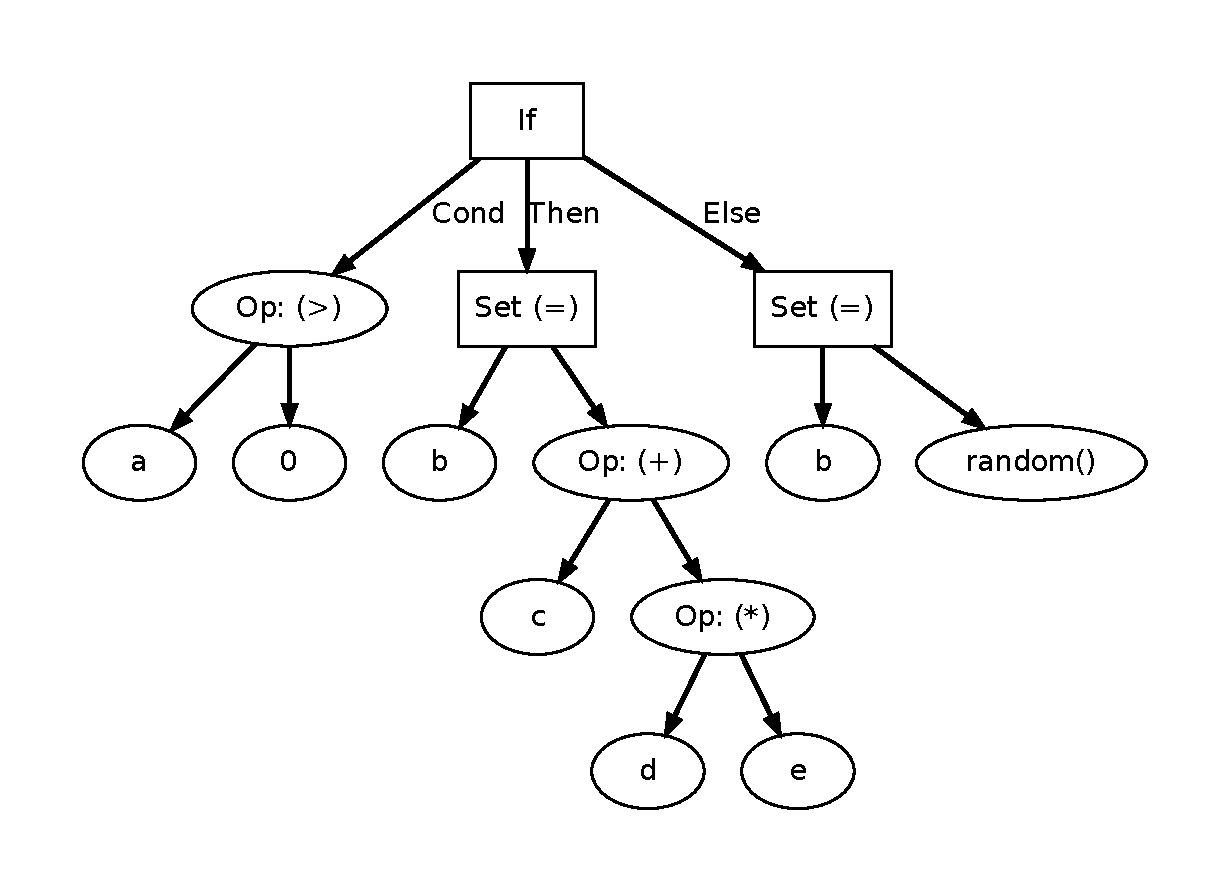
\includegraphics[width=\textwidth]{images/If.pdf}
        \caption{Пример AST}
        \label{fig:ast}
    \end{figure}
\end{center}

Программный код на языке {\sf C++} представим в виде AST (Abstract Syntax Tree~--- Абстрактное синтаксическое дерево).
AST программного кода~--- дерево, узлами которого являются операторы языка программирования или операции, а листьями~--- операнды (рис.\ref{fig:ast}). Реализация операций и операндов уже описана в прошлой главе~(\ref{sec:AST}). В этой главе рассмотрим реализацию операторов языка программирования {\sf C++}.

Оператор в императивных языках программирования (коим является {\sf C++})~--- это наименьшая автономная часть языка программирования; команда. В таблице~\ref{tab:stms} приведены примеры различных операторов на языке {\sf C++}.
\begin{table}
    \begin{center}
        \begin{tabular}{|l|l|}
            \hline
            Оператор & Пример\\
            \hline
            Объявление & \verb"int a = 0;"\\
            \hline
            Присваивание & \verb"a = b + c;" \\
            \hline
            Последовательность операторов & \verb"int a;" \\
                                          & \verb"a = b + c;"\\
            \hline
            Блок операторов &\verb"{" \\
                            &\verb"    int a;" \\
                            &\verb"    a = b + c;"" \\
                            &\verb"}" \\
            \hline
            Условный оператор & \verb"if (a != b){" \\
                              & \verb"    d = c + 1;" \\
                              & \verb"} else {" \\
                              & \verb"    d = c + 2;" \\
                              & \verb"}"\\
            \hline
            Оператор переключения & \verb"switch (a){" \\
                                  & \verb"    case 0:" \\
                                  & \verb"        d = c + 1;" \\
                                  & \verb"        break;" \\
                                  & \verb"    case 1:" \\
                                  & \verb"        d = c + 2;" \\
                                  & \verb"        break;" \\
                                  & \verb"}"\\
            \hline
            Цикл For & \verb"for(int i = 0; i < N; ++i){" \\
                     & \verb"    d+=i;" \\
                     & \verb"}" \\
            \hline
            Цикл с предусловием & \verb"while (a<10){" \\
                                & \verb"    a++;" \\
                                & \verb"}" \\
            \hline
            Цикл с постусловием & \verb"do {" \\
                                & \verb"    a++;" \\
                                & \verb"while (a<10);" \\
            \hline
            Вызов подпрограммы & \verb"IncreaseTemp(10);" \\
            \hline
            Возврат из подпрограммы & \verb"return 0;"\\
            \hline
        \end{tabular}
    \end{center}
    \caption{Различные виды операторов языка {\sf C++}}
    \label{tab:stms}
\end{table}

Хоть AST~--- дерево, набор операторов также представим в виде последовательно идущего программного кода~--- трассы выполнения программы. Это наиболее привычный вид, который используется при написании программы человеком~--- последовательно строчку за строчкой добавлять операторы в трассу выполнения программы. Этот принцип взят за основу кодогенерации в системе {\sf Symbalg}. 

Система {\sf Symbalg} реализована на языке программирования {\sf Python}, и используется в рамках синтаксиса языка {\sf Python}. Соответственно все использование системы должно вестись в рамках синтаксиса языка {\sf Python}, не используя дополнительные файлы с псевдокодом, и ограничивая использование строковых конструкций. {\sf Python}~--- объектно-ориентированный язык программирования, и все сущности представляют собой объекты~--- экземпляры классов. Операторы реализованы как классы языка {\sf Python}, и их экземпляры можно создавать при помощи явного использования конструкторов. Этот метод создания AST, несомненно, является громоздким и нежелательным. Для создания AST путем наполнения трассы выполнения программы были сформулированы следующие постулаты, на которых основана идеология системы кодогенерации:

\begin{enumerate}
    \item Хранение AST в виде дерева, узлами и листьями которого являются экземпляры классов системы {\sf Symbalg}.
    \item Возможность создания дерева с нуля, наполняя трассу выполнения программы в рамках синтаксиса языка {\sf Python}.
    \item Возможность гибко работать с уже созданным фрагментом AST, как с традиционным деревом (создание нового дерева на основе существующего(их), добавление ветвей, замена ветвей, удаление ветвей, рекурсивный перебор всех элементов дерева и т.д.).
\end{enumerate}

Опишем реализацию сформулированных постулатов по пунктам.

\subsection{Иереахия классов, реализующих операторы}

Базовым классом для операторов является \verb"BaseStm" и основная логика операторов описана в модуле \verb"statement.py". 
На рисунке~\ref{fig:hier} представлены классы, которые реализуют поведение операторов.

\begin{center}
    \begin{figure}
        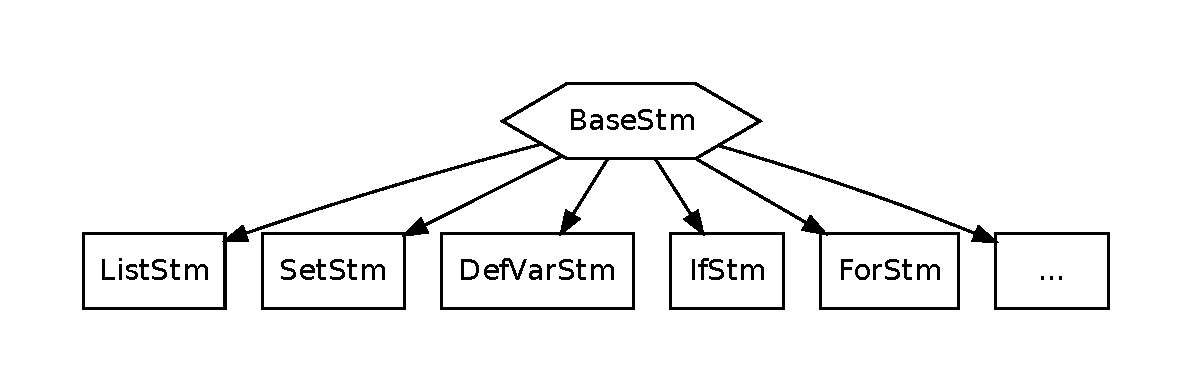
\includegraphics[width=\textwidth]{images/Hier.pdf}
        \caption{Иерархия классов, реализующих операторы}
        \label{fig:hier}
    \end{figure}
\end{center}

Каждый наследник класса \verb"BaseStm" реализует один из операторов, приведенных в таблице~\ref{tab:stms}. В таблице~\ref{tab:clstms} представлено сопоставление операторов и классов, их реализующих.
\begin{table}
    \begin{center}
        \begin{tabular}{|l|l|l|}
            \hline
            Оператор & Класс, реализующий                   & Описание класса\\
                     & оператор                             &\\
                                                           &&\\         
            \hline
            Объявление & \verb"DefVarStm"                   &Имеет поля \verb"name", \verb"type" и \verb"value"\\
            \hline
            Присваивание & \verb"SetStm"                    &Имеет поля \verb"lvalue", \verb"op" и \verb"expr"\\
            \hline
            Последовательность & \verb"ListStm"             &Имеет поле \verb"_list"~--- список операторов\\
            операторов         &                            &\\
            \hline
            Блок операторов &\verb"Пока не реализован"      &\\
            \hline
            Условный оператор & \verb"IfStm"                &Имеет поля \verb"cond", \verb"mode", \verb"_then" и \verb"_else"\\
                                                           &&Может работать в двух режимах: \\         
                                                           &&1) Только ветвь True (\verb"mode==True"),   \\         
                                                           &&2) Ветвь True и одна ветвь Else (\verb"mode==False"),   \\         
            \hline
            Оператор     & \verb"Пока не реализован"        &\\
            переключения &                                  &\\
            \hline
            Цикл For & \verb"ForStm"                        &Имеет поля \verb"init", \verb"cond", \verb"step" и \verb"code"\\
            \hline
            Цикл с предусловием & \verb"Пока не реализован" &\\
            \hline
            Цикл с постусловием & \verb"Пока не реализован" &\\
            \hline
            Вызов подпрограммы & \verb"Пока не реализован"  &\\
            \hline
            Возврат из   & \verb"Пока не реализован"        &\\
            подпрограммы &                                  &\\
            \hline
        \end{tabular}
    \end{center}
    \caption{Различные виды операторов языка {\sf C++}}
    \label{tab:clstms}
\end{table}

Эта иерерахия и лежит за реализацией первого пункта постулатов из трех.

\subsection{Заполнение AST путем наполнения трассы выполнения программы}
Второй постулат заключается в том, чтобы существовала возможность создания AST путем набирания трассы выполнения кода программы на языке {\sf C++} в рамках синтаксиса языка {\sf Python}. 
Первое, на чем нужно условиться, это то, что участок AST представляется в системе {\sf Symbalg}, как экземпляр класса \verb"ListStm".
Таким образом, в системе {\sf Symbalg}, наполнение трассы выполнения программы заключается в формировании списка операторов, который хранится в экземпляре класса \verb"ListStm".

Для этого функционала нам нужно по особому обрабатывать код на языке {\sf Python}, который будет составлять желаемый участок AST. 
Такая обработка кода в системе {\sf Symbalg} достигается путем исполнения участка кода на языке {\sf Python} в искусственно созданном пространстве имен. 

В этом пространстве имен нам хотелось бы легко вводить участок AST, то есть:
\begin{itemize}
    \item Использовать переменные внутри выражений без их изначального инициализирования
    \item Позволить вводить некоторые специфичные для языка {\sf C++} конструкции (циклы For, i++ и т.д) в синтаксисе языка {\sf Python}
    \item Просто вводить AST как программный код без самостоятельного создания каких-либо объектов.
\end{itemize}

Для этого предлагается реализовать класс, эмулирующий пространство имен~--- \verb"NamespaceStm".
Чтобы выполнить некий фрагмент кода в нужном пространстве имен, нужно этот фрагмент кода в виде строки передать в процедуру 
\verb"exec", а также в качестве локального пространства имен передать нужное нам пространство имен.
Для того, чтобы это можно было сделать, для этого класса, реализующего пространство имен нужно создать методы \verb"__getitem__" и \verb"__setitem__", которые используется в традиционных пространств имен (обычные словари) для возврата элемента по имени. 
Тем самым, вместо возврата элемента словаря в методе \verb"__getitem__" мы можем обрабатывать пришедшую на вход строку как угодно и совершать любые действия. Метод \verb"__setitem__" вызывается при конструкциях типа:
\begin{verbatim}
a = ...  # вызовет .__setitem__("a")
\end{verbatim}
Будем различать несколько типов переменных во фрагменте кода, представляющего участок AST:
\begin{itemize}
    \item переменная \verb"_"~--- при встрече с такой переменной создастся экземпляр класса \verb"EmptyVar".
    \item переменная, начинающаяся со знака подчеркивания~--- переменная, которая не войдет в AST и используется как обычная переменная языка {\sf Python}.
    \item переменная, не начинающаяся со знака подчеркивания~--- для нее создастся (если уже не был создан) экземпляр класса \verb"var".
    \item зарезервированная {\sf Symbalg} переменная для написания некоторых операторов (например~--- \verb"For", \verb"If", ...). При их встрече в коде, происходит создание экземпляра класса соответствующего оператора.
\end{itemize}

Для того, чтобы реализовать описанный функционал, был реализован декоратор \verb"@statement". При декорации им метода, все, что является телом этого метода передается в виде строки в процедуру \verb"exec" с локальным пространством имен \verb"NamespaceStm". 

Пример создания участка AST при помощи метода, декорируемого декоратором \verb"@statement":
\begin{verbatim}
@statement
def test():
    a[0,1,2] = w//b[2,3]
    For[i:0,N]
    a[1,3,4] = g[1,2,3]
\end{verbatim}

При вызове полученной функции возвращается экземпляр класса \verb"ListStm", с именем \verb"test". При вызове этого метода в качестве именованных аргументов можно передавать пары "переменная" : "операция". При этом во всем участке AST совершится подстановка предложенной операции вместо предложенной переменной.

В таблице~\ref{tab:examstms} приведены примеры использования операторов языка {\sf C++} внутри функций, декориуемых декоратором \verb"@statement".

\begin{table}
    \begin{center}
        \begin{tabular}{|l|l|}
            \hline
            Оператор & Пример\\
            \hline
            Объявление & \verb"В явном виде не реализован"\\
            \hline
            Присваивание & \verb"a = 1" \\
                         & \verb"----------------------------------------------" \\
                         & \verb"b += 1" \\
            \hline
            Последовательность операторов & \verb"a = 1" \\
                                          & \verb"b += 1" \\
            \hline
            Блок операторов &\verb"Пока не реализован" \\
            \hline
            Условный оператор & \verb"If[a>b]"\\
                              & \verb"c+=1"\\
                              & \verb"Else"\\
                              & \verb"c+=2"\\
                              & \verb"End"\\
            \hline
            Оператор переключения & \verb"Пока не реализован"\\
            \hline
            Цикл For & \verb"For[counter:start, stop]" \\
                     & \verb"B += counter"\\
                     & \verb"End"\\
                     & \verb"----------------------------------------------" \\
                     & \verb"For[counter:start, stop, step]"\\
                     & \verb"B /= counter"\\
                     & \verb"End"\\
                     & \verb"----------------------------------------------" \\
                     & \verb"For[counter, start, condition, nextstep]"\\
                     & \verb"B += counter"\\
                     & \verb"End"\\
                     & \verb"----------------------------------------------" \\
                     & \verb"For[type, counter, start, condition, nextstep]"\\
                     & \verb"B += counter"\\
                     & \verb"End"\\
            \hline
            Цикл с предусловием & \verb"Пока не реализован" \\
            \hline
            Цикл с постусловием & \verb"Пока не реализован" \\
            \hline
            Вызов подпрограммы & \verb"Пока не реализован" \\
            \hline
            Возврат из подпрограммы & \verb"Пока не реализован"\\
            \hline
        \end{tabular}
    \end{center}
    \caption{Пример реализации операторов языка {\sf C++}}
    \label{tab:examstms}
\end{table}

\subsection{Работа с AST как с деревом}
С участком AST(экземпляром класса \verb"ListStm") можно совершать различные действия. Для класса \verb"ListStm" определено сложение, которое интерпретируется как послеследование одного участка AST за другим. Уже существующий экземпляр класса \verb"ListStm" можно использовать как внутри пространства имен \verb"NamespaceStm", так и вне его. Использовать внутри \verb"NamespaceStm" можно при помощи следующей конструции:
\begin{verbatim}
_[StmName()] 
\end{verbatim}
При обращении к оператору, в круглых скобках можно указывать аргументы. При их помощи можно совершать изменения в AST, которое интерпретируется этим оператором. Есть два различных вида аргументов:
\begin{itemize}
    \item именованные аргументы, передаваемые при вызове экземпляра класса \verb"ListStm", используемые для макроподстановок. Например конструкция:
    \begin{verbatim}
StmName(a=b)
    \end{verbatim}
заменит все переменные \verb"a" внутри AST на переменную \verb"b"
    \item именованный аргумент \verb"_conv=func"~--- позволяет рекурсивно применять метод \verb"func" ко всем узлам AST. Метод может как собирать информацию с AST, так и изменять его части. Пример рекурсивной функции и ее применения:
    \begin{verbatim}
def offset_1(x):
    if isinstance(x, IndexOp) and type(x.b) is tuple:
        x.b = tuple([i+1 for i in x.b])
    return x

print StmName()(_conv=offset_1)    
    \end{verbatim}
    Эта функция прибавляет единицу ко всем, встречающимся в AST, индексам (содержимым квадратных скобок)
\end{itemize}
\[
    
\]
\end{document}
